\documentclass{article}
\title{Tapis Roulant}
\author{Elara Onno et Héléna Benet Burgaud}
\date{\today}

\usepackage[a4paper]{geometry}
\geometry{left=2.5cm, top=2.5cm, right=2.5cm, bottom=2.5cm, bindingoffset=0mm}
\usepackage{graphicx}
\usepackage{subcaption}
\usepackage{parskip}
\usepackage{enumitem} % joli pour lister
\usepackage{esvect} %\vv : for vectors
\usepackage{empheq} % : for cases
\usepackage{amsmath} % \alignat
\usepackage{amssymb} % \mathbb
\usepackage{changepage} % \adjustwidth
\usepackage[french]{babel}
\usepackage{accents}
\usepackage{xcolor}
\usepackage{array}
%%%%%%%%%%%%
\usepackage[colorlinks, linkcolor=black]{hyperref}
%%%%%%%%%%%%
\newcolumntype{C}[1]{>{\centering\arraybackslash }b{#1}}
%%%%%%%%%%%%
\definecolor{myblue}{RGB}{42, 110, 190}
\definecolor{mycyan}{RGB}{100, 190, 180}
\definecolor{background}{RGB}{240, 240, 240}
\definecolor{violet}{RGB}{83,0,83}

\usepackage{listings}
\usepackage{tikz}
\lstset{
	language=Octave,
	backgroundcolor=\color{background},
	keywordstyle=\bf\color{myblue},
	numberstyle=\color{gray},
	identifierstyle=\color{black},
	commentstyle=\color{mycyan},
	tabsize=3,
	breaklines=true,
	postbreak=\mbox{\textcolor{red}{$\hookrightarrow$}\space},
	prebreak=\mbox{\textcolor{red}{$\hookleftarrow$}\space},
	basicstyle= \ttfamily,
  	literate={+}{{\textcolor{myblue}{+}}}1
           {-}{{\textcolor{myblue}{-}}}1
           {*}{{\textcolor{myblue}{*}}}1
           {=}{{\textcolor{myblue}{=}}}1
           {<}{{\textcolor{myblue}{<}}}1
           {>}{{\textcolor{myblue}{>}}}1
           {;}{{\textcolor{myblue}{;}}}1
           {,}{{\textcolor{myblue}{,}}}1
           {octave}{{\textcolor{myblue}{\bf{octave}}}}7
           }
%%%%%%%%%%%%
\newcommand{\ts}{\scriptscriptstyle}
\newcommand{\ds}{\displaystyle}

%\setcounter{section}{-1}

\begin{document}
\maketitle
\tableofcontents
\newpage

\noindent Le système $\Sigma_1$ que nous étudierons est composé d'un solide posé sur un tapis roulant de vitesse constant $\vec{v}$. Celle-ci est accrochée à un ressort lui même fixé sur un plan vertical. 

\begin{figure}[h!]
	\centering
	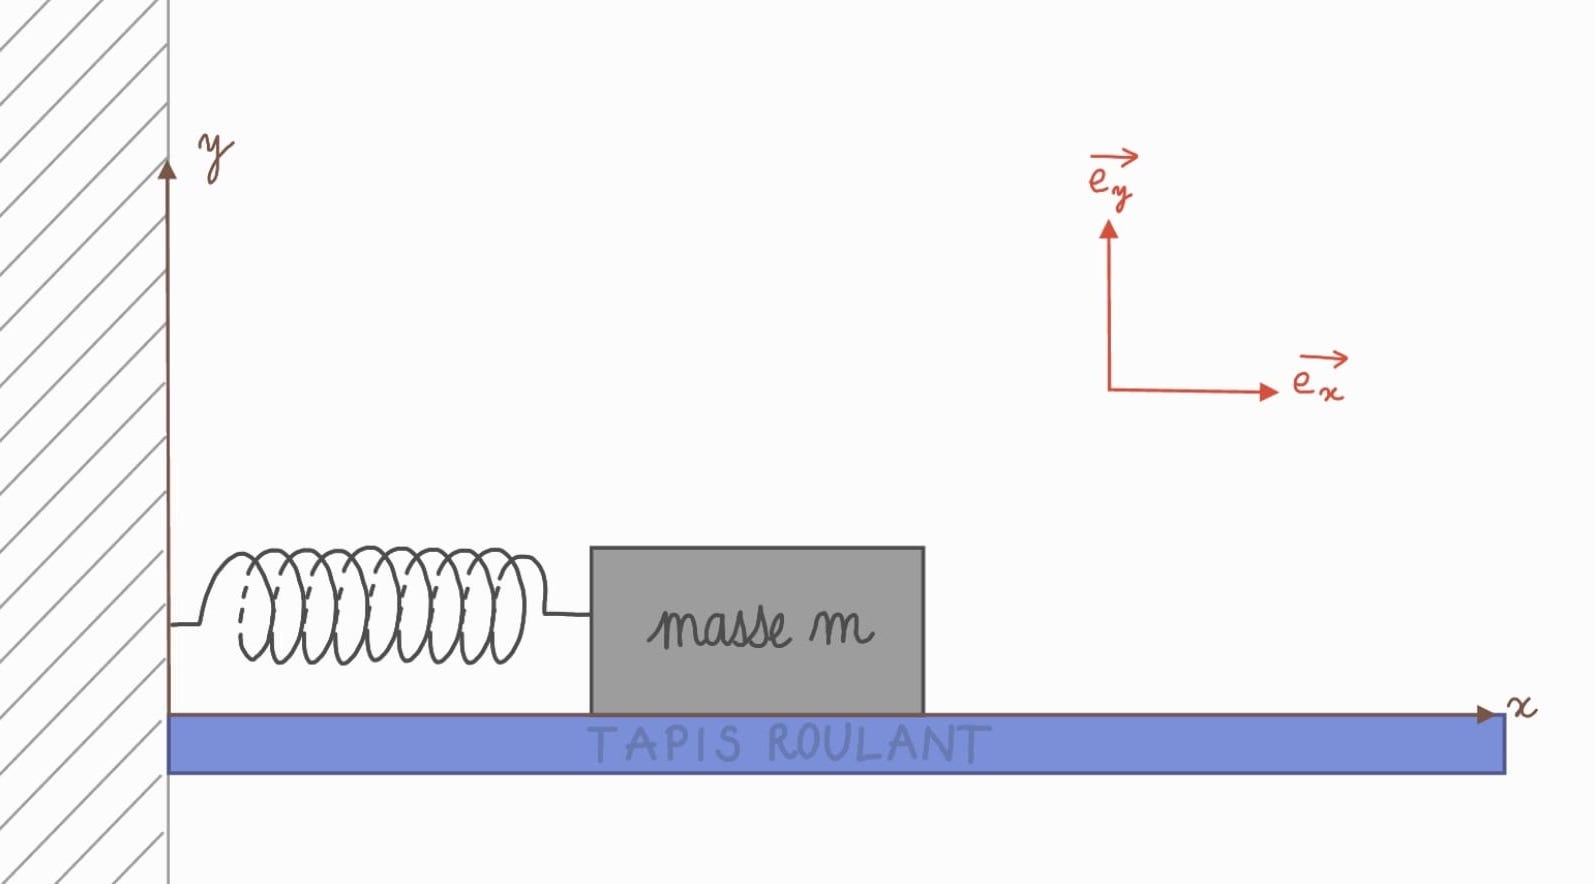
\includegraphics[scale=.26]{sch1.jpg}
	\caption{Système $\Sigma_1$}
\end{figure}
Dans ce chapitre nous allons modéliser la position de la masse en fonction du temps. Pour cela, nous allons présenter ultérieurement les 3 cas que l'on traitera.

\section{Introduction}\label{sec_1}
\paragraph{Variables du problème}\label{par_1.0.0.1}

\begin{adjustwidth}{0cm}{6cm}
\vspace{-.7cm}
\begin{alignat*}{2}
k \quad&[N\cdot m^{-1}] &&\quad \text{la raideur du ressort}\\
l_0  \quad&[m] &&\quad \text{la longueur du ressort} \\
m \quad&[g] && \quad\text{la masse du solide}\\
g \quad&[m\cdot s^{-2}] &&\quad \text{qui caractérise le champ gravitationnel} \\
\text{v} \quad& [m\cdot s^{-1}] && \quad\text{la vitesse du tapis roulant} \\
v_0 \quad& [m\cdot s^{-1}] && \quad\text{la vitesse initiale de la masse} \\
\nu \quad&[\text{sans unité}] && \quad\text{les frottements crées par le tapis roulant} 
\end{alignat*}
\end{adjustwidth}

%Dans notre étude, tous nos résultats seront selon ces six variables
\paragraph{Cinématique de la masse}\label{par_1.0.0.2}
\begin{alignat*}{3}
& \vv{OM} \quad && = \quad  x(t)~\vv{e_x}\\
\intertext{sa vitesse :}
& \vv{v}(M) \quad && = \quad  \dot{x}(t)~\vv{e_x}\\
\intertext{et son accélération :}
& \vv{a}(M) \quad && = \quad  \ddot{x}(t)~\vv{e_x}
\end{alignat*}

\paragraph{Efforts extérieurs}\label{par_1.0.0.3}
%
\begin{adjustwidth}{0cm}{3.5cm}
\vspace{-.7cm}
\begin{alignat*}{3}
& \vv{P} \quad && = \quad  -mg~\vv{e_y} &&\qquad \text{le Poids}\\
& \vv{R} \quad && = \quad  R~\vv{e_y} &&\qquad \text{la Réaction du tapis roulant}\\
& \vv{F_k} \quad && = \quad  -k(x(t)-l_0)~\vv{e_x} &&\qquad \text{la Force de rappel exercée par le ressort}\\
& \vv{F_{\ts{T}}} \quad && = \quad  F_{\ts{T}}~\vv{e_x} &&\qquad \text{la Force d'entraînement du tapis roulant}
\end{alignat*}
\end{adjustwidth}
%
\paragraph{Principe fondamental de la dynamique (Deuxième loi de Newton)}\label{par_1.0.0.4}
%
\begin{alignat}{2}
\sum{\vv{F}} &=  m\vv{a}\nonumber\\
\intertext{Suivant $\vv{e_y}$ :} \nonumber
 R- mg \quad & =  \quad 0 \nonumber\\
 R  \quad & = \quad  mg \nonumber\\
\intertext{Suivant $\vv{e_x}$ :} \nonumber \\
-k(x-l_0)+F_{\ts{T}}(t)\quad & = \quad m\ddot{x} \label{eq_1}
\end{alignat}
%
\subsection{Un système à deux régimes}\label{ssec_1.1}
Dans le mouvement de ce système, on distingue deux régimes spécifiques. Un premier régime, le régime d'adhérence ou la masse adhère à la surface du tapis roulant et est entrainée par celui-ci. Un second régime, le régime de glissement dans lequel la masse n'adhère plus au tapis roulant : elle glisse. Chacun de ces régimes est déterminé par des conditions particulières : on a à la fois des conditions initiales en position et en vitesse mais aussi une condition sur la force d'entraînement du tapis roulant sur l'ensemble de la phase sous ce régime. 

\subsubsection{Conditions sur les régimes}\label{sssec_1.1.1}

\paragraph{Régime d'adhérence}\label{par_1.1.1.1}
\mbox{}\\
Pour être en régime d'adhérence, les conditions initiales (à l'instant initial $t_d$ du régime) doivent respecter des contraintes particulières.
%
\begin{align*}
\begin{cases}
\vspace{.2cm}
x(t_d)\;=\; x_d\;=\; l,\quad l\in [l_0-\alpha~,~l_0+\alpha]\\
\dot{x}(t_d)\;=\;\text{v} 
\end{cases}
\end{align*}
%
Ici, l'intervalle $[l_0-\alpha~,~l_0+\alpha]$ est un intervalle particulier qui respecte les conditions d'adhérence. Plus précisément, si on se trouve à la position limite $l_0+\alpha$, le ressort est très tendu, donc au-delà de cette valeur, on passe à un régime de glissement ; à l'inverse, si on se trouve en $l_0-\alpha$, le ressort est très compressé donc ici encore, au-delà de cette valeur, on se trouve en régime de glissement. On verra dans la suite comment évaluer la valeur de $\alpha$.

De plus, la vitesse de la masse en régime d'adhérence correspond forcément à v, la vitesse d'entraînement du tapis roulant.   

On a aussi une condition sur la force d'entraînement du tapis sur l'ensemble du régime d'adhérence :
%
\begin{equation}
\mid F_{\ts{T}}(t) \mid  \quad<\quad F_c \quad=\quad\nu\; R \label{eq_2}
\end{equation}
%
\paragraph{Régime de glissement}\label{par_1.1.1.2}
\mbox{}\\
D'après ce qu'on a vu pour le régime d'adhérence, les conditions initiales pour se trouver en régime de glissement sont les conditions contraires aux conditions initiales d'adhérence :
%
\begin{align*}
\begin{cases}
\vspace{.2cm}
x(t_d)\;=\;x_d\;=\;l,\quad l\notin [l_0-\alpha~,~l_0+\alpha]\\
\dot{x}(t_d)\;=\;v_d\;\neq\; \text{v}
\end{cases}
\end{align*}
%
Ici, l'une des deux conditions suffit à être en régime de glissement (contrairement à précédemment où les deux conditions devaient être vérifiées).  

La condition sur l'ensemble de la phase pour la force est :
$$\mid F_{\ts{T}}(t)\mid\quad=\quad F_c$$
%
\subsubsection{Généralités sur le mouvement suivant le régime}\label{ssseq_1.1.2}
On va maintenant préciser l'équation du mouvement de la masse suivant le régime dans lequel elle se trouve. 

\paragraph{Régime d'adhérence}\label{par_1.1.2.1}
\mbox{}\\
Pour ce régime, la vitesse de la masse est constante et correspond à la vitesse du tapis roulant. On a donc :
\begin{alignat}{2}
& &\dot{x}(t)\quad & =\quad \text{v}~,\text{v}\in\mathbb{R} \nonumber\\
&\text{donc :} \quad & \ddot{x}(t)\quad & = \quad 0 \nonumber\\
&\text{et donc :} \quad & F_{\ts{T}}(t)\quad &= \quad k(x(t)-l_0) \quad \text{d'après le PFD} \nonumber\\
\intertext{En définissant $t_d$ comme l'instant initial du régime, on a finalement : }
& & \quad x(t) \quad &= \quad x(t_d)+(t-t_d)\;\text{v} \label{eq_3}
\end{alignat}
 %
\paragraph{Régime de glissement}\label{par_1.1.2.2}
\mbox{}\\
On cherche une expression de $x$ en fonction du temps en régime de glissement.D'après le PFD (vu précédemment), $x$ en régime de glissement est solution de l'équation différentielle qui suit :

\begin{equation}
m\ddot{x}(t)+kx(t)\quad=\quad k\;l_0 \pm F_c \label{eq_4}\\
\end{equation}

On résout cette équation différentielle. L'équation homogène associée est : 
\begin{alignat}{3}
& \quad & m\ddot{x}(t)+kx(t) \quad & = \quad 0 \label{eq_5}\\
& \Longleftrightarrow \quad & \ddot{x}(t)-\dfrac{k}{m}x(t)\quad & = \quad 0 \nonumber
\end{alignat}

Les solutions générales de cette équation \eqref{eq_5} sont :
%
\begin{align*}
x_h(t) \quad=\quad A\cos(\omega (t-t_d))+B\sin( \omega (t-t_d)) 
\end{align*}

Avec $A$, $B$ $\in \mathbb{R}$ et $\omega = \sqrt{\dfrac{k}{m}}$ et $t_d$ désignant l'instant initial du régime de glissement.  

On cherche maintenant une solution particulière de \eqref{eq_4}. Une solution évidente est : 

$$x_e(t)\quad =\quad l_0 \pm \dfrac{F_c}{k}$$

Donc l'ensemble des solutions de \eqref{eq_4} est :
\begin{align}
	x(t)& \quad=\quad x_h(t)+x_e(t)\nonumber\\
	&\quad=\quad A\cos(\omega (t-t_d))+B\sin (\omega (t-t_d)) +l_0 \pm \dfrac{F_c}{k} \label{eq_6}
\end{align}
Déterminons A et B.

Nous avons les conditions initiales suivantes : 

\begin{align*}
&\quad\begin{cases}
\vspace{.2cm}
	x(t_d)& \;=\; \quad x_d\\
	\dot{x}(t_d) & \;=\; \quad v_d 
\end{cases}
\\\\
\intertext{On rappelle que : 
$\dot{x}(t)=B\omega\cos(\omega (t-t_d) - A\omega \sin(\omega (t-t_d))$.
Donc en remplaçant $x(t_d)$ et $\dot x(t_d)$ par leur expressions, on obtient :}
\end{align*}
\begin{align*}
&\quad
\begin{cases}
\vspace{.2cm}
x(t_d) &= \quad A + l_0 \pm \dfrac{F_c}{k} = x_d \\
\dot{x}(t_d) &= \quad B\; \omega = v_d  
\end{cases}	\\\\
\Longleftrightarrow
&\quad
\begin{cases}
\vspace{.2cm}
A + l_0 \pm \dfrac{F_c}{k} \quad &= \quad x_d  \\
\hfill B\;\omega \quad &= \quad v_d 
\end{cases}	\\\\
\Longleftrightarrow
&\quad
\begin{cases}
\vspace{0.2cm}
	A \quad &= \quad x_d- \Big{(}l_0 \pm \dfrac{F_c}{k}\Big{)} \qquad(7)\\
	B  \quad &= \quad \dfrac{v_d}{\omega} \qquad \hfill(8)
\end{cases}	
\end{align*}

Si on injecte les expressions de $A$ et $B$ dans \eqref{eq_6}, on obtient :

\begin{align}
	x(t) \quad&=\quad A\cos(\omega (t-t_d))+B\sin(\omega (t-t_d))+ l_0 \pm \dfrac{F_c}{k} \nonumber \\
	&= \quad\left(x_d - \Big{(}l_0 \pm \dfrac{F_c}{k}\Big{)}\right)\cdot\cos(\omega (t-t_d)) +\dfrac{v_d}{\omega}\cdot\sin(\omega (t-t_d)) + l_0 \pm \dfrac{F_c}{k}\addtocounter{equation}{2} \label{eq_7}
\end{align}

\subsection{Cas traités}\label{ssec_1.2}
On va traiter quatre cas différents de phase initiale. Ces quatre cas constituent l'ensemble des possibilités pour les conditions initiales en $t_0$, instant initial du mouvement.  
\paragraph{Cas 1 (Régime initial d'adhérence)}\label{par_1.2.0.1}
\mbox{}\\
Le premier cas, le plus simple, est régi par les conditions initiales suivantes :
$$
\begin{cases}
	\vspace{.2cm}
	x_0\;\in\; [l_0-\alpha~,~l_0-\alpha]\\
	v_0 \;=\; \text{v}
\end{cases}
$$
C'est le seul cas pour lequel on débute par une phase d'adhérence. 

\paragraph{Cas 2 (Régime initial de glissement)}\label{par_1.2.0.4}
\mbox{}\\
Le deuxième cas représente le cas contraire au premier.$$
\begin{cases}
	\vspace{.2cm}
	x_0 \quad\text\small{quelconque}\qquad \text\small{ou}\\
	v_0 \quad\text\small{quelconque}
\end{cases}
$$
Il se divise en trois sous cas :
\subparagraph{Cas 2.1}
$$
\begin{cases}
	\vspace{.2cm}
	x_0  \in [l_0-\alpha~,~l_0-\alpha]\\
	v_0 \neq \text{v}
\end{cases}
$$
\subparagraph{Cas 2.2}
$$
\begin{cases}
	\vspace{.2cm}
	x_0  \not\in [l_0-\alpha~,~l_0-\alpha]\\
	v_0 = \text{v}
\end{cases}
$$

\subparagraph{Cas 2.3}
$$
\begin{cases}
	\vspace{.2cm}
	x_0  \not\in [l_0-\alpha~,~l_0-\alpha]\\
	v_0 \neq \text{v}
\end{cases}
$$
\newpage
\section{Démarche}\label{sec_2}
\subsection{Fonctions utilisées}\label{ssec_2.1}
Comme on a vu dans \ref{ssec_1.1} on a deux régimes, le régime d'adhérence et celui de glissement. On définit donc pour chacun des régimes une fonction de la position : 

\begin{lstlisting}
% Position dans un regime de glissement
function x = xG(t,t_d,x_d,v_d,v,omega,phi)
  x = (x_d - phi) * cos(omega * (t - t_d)) + v_d/omega * sin(omega * (t - t_d)) + phi;
endfunction
\end{lstlisting}

\begin{lstlisting}
% Position dans un regime d'adherence
function x = xA(t,t_d,x_d,v)
  x = v * (t - t_d) + x_d;
end
\end{lstlisting}

Dans les deux fonctions on a plusieurs arguments, \verb|t_d|, \verb|x_d|, \verb|v_d| qui sont des variables initiales au régime; v qui est la vitesse du tapis, enregistrée dans les variables d'entrée; finalement, on a \verb|omega| et \verb|phi| qui sont des variables intermédiaires. \\
\begin{lstlisting}
function [k,l_0,m,g,v,nu]=VarEntree
	k = 20;		% cst raideur ressort    	[N/m]
	l_0 = .3;	% long a vide ressort    	[m]
	m = .1;		% masse                  	[kg]
	g = 9.81;	% cst gravitation        	[m/s^2]
	v = .1;		% vitesse tapis          	[m/s]
	nu = 1;		% adherence tapis        	[]
endfunction
\end{lstlisting}

\begin{lstlisting}
function [F_c,omega,tcF,tcK]=VarInter(k,l_0,m,g,v,nu)
	F_c = nu*m*g;      % max Force entrainement					[N]
	omega = sqrt(k/m); % Pulsation									[1/s]
	tcF = F_c/(k*v);   % Temps carct deter par condition ini	[s]
	tcK = 2*pi/omega;  % Temps carct deter par pusation		[s]
endfunction
\end{lstlisting}

Le \verb|phi| utilisé dans la fonction \verb|xG| n'est pas une constante, on la définit comme $\varphi = l_0 \pm \dfrac{F_c}{k}$ avec le signe de $\dfrac{F_c}{k}$ dépendant de la différence de vitesse entre la masse et du tapis.

En effet, si la v$- v \geq 0$ alors v $\geq v$, c'est à dire que le tapis entraine la masse vers les x positifs. Ainsi on a $F_{\ts{T}}\geq0$. Dans le cas contraire, la masse a une vitesse plus élevée que celle du tapis et donc le tapis exerce une force vers les x négatifs. On aura donc $F_{\ts{T}}\leq0$.

Ainsi on définit une fonction \verb|Phi| qui dépend de la vitesse du tapis et celle de la masse au début de chacun des régimes.

\begin{lstlisting}
function phi = Phi(v_d,k,l_0,v,F_c)
  if(v_d != v)
    s = - sign(v_d - v);
  else
    s = 1;
  end
  phi = l_0 + s * F_c/k;
endfunction
\end{lstlisting}

\subsection{Recherche des temps de changement de régime}\label{ssec_2.2}
\subsubsection{Temps de passage : Adhérence $\rightarrow$ Glissement}\label{sssec_2.2.1}
On va dans un premier temps chercher l'instant $t$ tel qu'on passe de régime d'adhérence en régime de glissement. 

Comme on a vu dans \ref{par_1.1.1.1}, pour rester en régime d'adhérence, il faut satisfaire la condition \eqref{eq_2}. Ainsi, pour passer d'un régime d'adhérence à un régime de glissement il faut que: $\mid F_{\ts{T}}\mid = F_c$.

De fait, on définit la fonction \verb|fT| modélisant la force du tapis.
\begin{lstlisting}
function f = fT(t,t_d,x_d,v_d,v,k,l_0,F_c,re)
  if(v_d != v)
    s = - sign(v_d - v);
  else
    s = 1;
  end
  %
  if(re == 'ad')
    x = xA(t,t_d,x_d,v);
    f = k * (x - l_0);
  elseif(re == 'gl')
    f = s * F_c;
  end
end
\end{lstlisting}

On peut de la même manière définir la fonction \verb|fK| qui représente la force exercée par le ressort.
\begin{lstlisting}
function f = fK(t,t_d,x_d,v_d,v,k,l_0,omega,phi,re)
  if(re=='ad')
    x = xA(t,t_d,x_d,v);
  elseif(re=='gl')
    x=xG(t,t_d,x_d,v_d,v,omega,phi);
  end
   f = - k * (x - l_0);
endfunction
\end{lstlisting}

Pour donner une estimation de $t$, on a deux options : par le calcul analytique (grâce à l'égalité \eqref{eq_3}) ou par un calcul de racine de la fonction $\mid F_{\ts T}\mid -\; F_c$.

La relation \eqref{eq_3} nous permet de dire que 
\begin{align}
k(x_d+(t_{d+1}-t_d)\;\text{v}-l_0) \quad &= \quad F_c \nonumber\\
\intertext{Et ainsi on a :}
x_d+t_{d+1}\text{v}-t_d\text{v}-l_0 \quad &= \quad \dfrac{F_c}{k}\nonumber\\
t_{d+1}\text{v}\quad &= \quad \dfrac{F_c}{k}-x_d+l_0+t_d\text{v}\nonumber\\
t_{d+1}\quad &=\quad \dfrac{1}{v}\left(\dfrac{F_c}{k}-x_d+l_0+t_d\text{v}\right)\nonumber\\
&=\quad t_d + \dfrac{F_c}{k\;v} - \dfrac{x_d - l_0}{v}
\end{align}

Ainsi on a :
\begin{lstlisting}
% Estimation numerique
CostA = @(t,t_d,x_d,v_d,v,k,l_0,F_c) (abs(fT(t,t_d,x_d,v_d,v,k,l_0,F_c,'ad')) - F_c).^2;
it1 = find(diff(sign(diff(CostA(t,t_0,x_0,v_0,v,k,l_0,F_c))))==2,1);
t_1 = fminsearch(@(t) CostA(t,t_0,x_0,v_0,v,k,l_0,F_c),t01(it1 + 1));
\end{lstlisting}
Avec \verb|x_0|, \verb|v_0|, \verb|t_0| les conditions initiales du régime d'adhérence et \verb|t_1| le temps de changement d'adhérence à glissement.

\subsubsection{Temps de passage : Glissement $\rightarrow$ Adhérence}\label{sssec_2.2.2}
Pour passer d'un régime de glissement à un régime d'adhérence, on revient aux conditions pour être en régime d'adhérence (dans \ref{par_1.1.2.1}), en particulier, on a besoin que $\dot x = $ v.
Ainsi on définit une fonction \verb|dxG| qui représente $\dot x$ en régime de glissement.
\begin{lstlisting}
function dot_x = vG(t,t_d,x_d,v_d,w,phi)
  dot_x = - (x_d - phi) * w * sin(w * (t - t_d)) + v_d * cos(w * (t - t_d));
endfunction
\end{lstlisting}

Il nous manque que à trouver numériquement la racine de la fonction $\dot x(t) -$v.
\begin{lstlisting}
% Estimation numerique
CostG = @(t,t_d,x_d,v_d,w,phi,v) ((vG(t,t_d,x_d,v_d,w,phi) - v).^2);
it1=find(diff(sign(diff(CostG(t01,t_0,x_0,v_0,w,phi,v))))==2,1);

t_1 = fminsearch(@(t) CostG(t,t_0,x_0,v_0,w,phi,v),t01(it1+1));
\end{lstlisting}

Avec, à nouveau, \verb|x_0|, \verb|v_0|, \verb|t_0| les conditions initiales du régime de glissement et \verb|t_1| le temps de changement de glissement à adhérence.

\newpage
\section{Cas 1}
On cherche à caractériser le mouvement de la masse, sa vitesse et la force d'entraînement du tapis en fonction du temps et d'en donner une représentation graphique dans le premier cas. Pour cela, on va d'abord déterminer les premiers temps $t_n$ de changement de régime.   
  
Comme énoncé précédemment, on se trouve dans les conditions initiales suivantes : 

$$
\begin{cases}
	\vspace{.2cm}
	x_0\in [l_0-\alpha~,~l_0-\alpha]\\
	v_0 = \text{v}
\end{cases}
$$

Le premier régime est alors un régime d'adhérence. Dans le code, on initialise de la même façon les variables initiales : 
\begin{lstlisting}
%% Variables d'initialisation
t_0 = 0 			% tmps ini		[s]
x_0 = l_0; 		% position ini	[m]
v_0 = v;			% vitesse ini	[m/s]       
\end{lstlisting}

Dans la suite du code, on utilisera toujours v directement. 


\subsection{Calcul de $t_1$ : Adhérence $\rightarrow$ Glissement}\label{ssec_3.1}
On va dans un premier temps chercher l'instant $t_1$ auquel le système va passer en régime de glissement. On a deux possibilités pour donner une estimation de $t_1$ : par le calcul analytique (grâce à l'égalité que l'on a montré précédemment) ou par un calcul de racine de la fonction $F_{\ts T}-F_c$. On va également comparer les résultats des deux méthodes par un calcul d'écart. Ceci nous donne le code suivant :

\begin{lstlisting}
% Estimation analytique de t1
t1A = t_0+tcF - (x_0 - l_0)/v;

% Estimation numerique de t1
Cost = @(t) (fT(t,t_0,x_0,v,v,k,l_0,F_c,'ad') - F_c).^2;
t1N = fminsearch(@(t) Cost(t), t_0 + tcK);

%Ecart :
ecart_t_1 = t1A-t1N
\end{lstlisting}

Pour le calcul de \verb|t1N|, on prend \verb|t_0 + tcK| comme point de départ de la recherche pour \verb|fminsearch(...)| car en théorie, cette valeur est proche de la valeur attendue pour $t_1$. 

Ici, on va plutôt choisir la valeur analytique de $t_1$ puisque le calcul est moins coûteux et demande moins d'approximations. On en déduit également une valeur de $x$ associée :
\begin{lstlisting}
t_1 = t1A
x_1 = xA(t_1,t_0,x_0,v)
\end{lstlisting}

\subsection{Calcul de $t_2$ : Glissement $\rightarrow$ Adhérence}
On passe ensuite en régime de glissement. On cherche maintenant à calculer $t_2$ : 

\begin{lstlisting}
% Estimation numerique de t2
Cost = @(t) abs(d_xG(t,t_1,x_1,v,omega,phi) - v);
t2N = fminsearch(@(t) Cost(t), t_1 + tcK)
\end{lstlisting}

Le choix de point de départ de recherche \verb|t_1 + tcK| dans le \verb|fminsearch(...)| est à nouveau choisi de sorte qu'il soit assez proche de $t_2$. 

On effectue également le calcul de $x$ associé à $t_2$ :

\begin{lstlisting}
t_2 = t2N
x_2 = xG(t_2,t_1,x_1,v,v,omega,phi)
\end{lstlisting}

A ce stade on a :

\begin{lstlisting}
>>
t_1 = 0.490491907097087

ecart_t_1=8.092902913481304e-06

t_2 = 0.934780200912923

x_1 = 0.349049190709709
x_2 = 0.349049190709709
\end{lstlisting}

L'écart entre les valeurs analytique et numérique de $t_1$ est très faible : utiliser l'une ou l'autre méthode pour les calculs n'aura pas beaucoup d'influence sur le résultat final. On remarque aussi que $x_1=x_2$.

\subsection{Calcul de $t_3$}
On répète l'opération pour $t_3$ : on passe en régime d'adhérence après $t_2$ et on effectue le calcul de $t_3$  de la même manière que l'on a fait le calcul de $t_1$. 
\begin{lstlisting}
% Estimation analytique de t3
t3A = t_2+tcF - (x_2 - l_0)/v;
t_3 = t3A
\end{lstlisting}
 
\subsection{Représentation graphique et résultats}
On a les valeurs suivantes pour $t_0$, $t_1$, $t_2$, $t_3$ :
\begin{lstlisting}
octave> main1
 t_0 = 0
 t_1 = 0.3270
 t_2 = 0.6898
 t_3 = 0.6898
\end{lstlisting}

On remarque ici que $t_2 = t_3$. On peut donc dire qu'après $t_2$ on passe en régime de glissement sans revenir au régime d'adhérence. En effet, la condition $F_{\ts{T}} = F_c$ est toujours vérifiée, donc aussitôt qu'on rentre en régime d'adhérence, on en sort.

On a donc les représentations graphiques suivantes pour le mouvement, la vitesse et les forces d'entraînement du tapis et de réaction du ressort : 

\begin{figure}[h!]
	\centering
	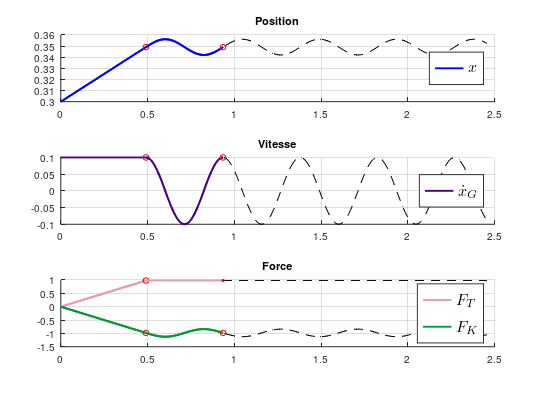
\includegraphics[scale=.6]{CAS1.png}
	\caption{Cas 1}
\end{figure}

\newpage

\section{Cas 2,3,4}
Comme dans le cas 1, on cherche à caractériser le mouvement de la masse, sa vitesse et la force d'entraînement du tapis en fonction du temps et d'en donner une représentation graphique dans le second cas énoncé. On donne d'abord les conditions initiales pour chaque cas :

\paragraph{Cas 2}
 
$$
\begin{cases}
	\vspace{.2cm}
	x_0 \in [l_0-\alpha~,~l_0-\alpha]\\
	v_0\neq \text{v}
\end{cases}
$$

Dans le code on note :

\begin{lstlisting}
%CAS 2
%Variables d'initialisation
t_0 = 0 			% tmps ini		[s]
x_0 = l_0; 		% position ini	[m]
v_0 = v + u;		% vitesse ini	[m/s]     
\end{lstlisting}

avec $u\in \mathbb{R}^*$ arbitraire.

\paragraph{Cas 3}

$$
\begin{cases}
	\vspace{.2cm}
	x_0 \notin [l_0-\alpha~,~l_0-\alpha]\\
	v_0= \text{v}
\end{cases}
$$

Dans le code :

\begin{lstlisting}
%CAS 3
%Variables d'initialisation
t_0 = 0				% tmps ini		[s]
x_0 = l_0 + d;		% position ini	[m]
v_0 = v ;			% vitesse ini	[m/s]       
\end{lstlisting}

avec $d\in \mathbb{R}^*$ aribitraire.

\paragraph{Cas 4}

$$
\begin{cases}
	\vspace{.2cm}
	x_0 \notin [l_0-\alpha~,~l_0-\alpha]\\
	v_0\neq \text{v}
\end{cases}
$$

Dans le code :

\begin{lstlisting}
%CAS 4
%Variables d'initialisation
t_0 = 0				% tmps ini		[s]
x_0 = l_0 + d;		% position ini	[m]
v_0 = v + u ;		% vitesse ini	[m/s]       
\end{lstlisting}

avec $d,~u\in \mathbb{R}^*$ arbitraires.

Avec ces conditions initiales, on commence en régime de glissement.

\subsection{Calcul de $t_1$ : Glissement $\rightarrow$ Adhérence}
On effectue le calcul de $t_1$ à partir de ce que l'on a défini dans la partie de recherche :

\begin{lstlisting}
% Estimation numerique de t_1
Cost = @(t) abs(d_xG(t,t_0,x_0,v_0,omega,phi) - v);
\end{lstlisting}

On a ensuite :
\paragraph{Cas 2}
$ $
\begin{lstlisting}
%CAS 2
t_1 = fminsearch(@(t) Cost(t), t_0 + 3/2 * tcK)		
\end{lstlisting}

\paragraph{Cas 3}
$ $
\begin{lstlisting}
%CAS 3
t_1 = fminsearch(@(t) Cost1(t),t_0 + 1/2 * tcK)		
\end{lstlisting}

\paragraph{Cas 4}
$ $
\begin{lstlisting}
%CAS 4
t_1 = fminsearch(@(t) Cost1(t),t_0 + tcK)		
\end{lstlisting}

Pour chacun des cas, on choisit le point de départ de la recherche du minimum par lecture graphique afin que dans chacun d'eux, la valeur choisie nous permette de tomber sur la bonne valeur de $t_1$ (le premier point qui vérifie la condition après $t_0$ dans le sens positif). 

Dans le même temps, on calcule $x(t_1)$ dans chaque cas en prenant $d=0.1$ et $u=0.2$ : 

\begin{lstlisting}
d = 0.1;
u = 0.2;
\end{lstlisting}

\paragraph{Cas 2}
$ $ 
\begin{lstlisting}
>>
t_1 = 0.424794257130005
x_1 = 0.296077798483522
\end{lstlisting}

\paragraph{Cas 3}
$ $ 
\begin{lstlisting}
>>
t_1 = 0.241675396907918
x_1 = 0.298102878339728
\end{lstlisting}

\paragraph{Cas 4}
$ $
\begin{lstlisting}
>>
t_1 = 0.703443567253337
x_1 = 0.294318109098953
\end{lstlisting}

\subsection{Calcul de $t_2$ : Adhérence $\rightarrow$ Glissement}\label{ssec_4.2}
Pour $t_2$, on se trouve dans la situation de passage entre adhérence et glissement : on a deux choix possibles pour le calcul de $t_2$. Ceux-ci sont analogues à ceux effectués en partie \ref{ssec_3.1}. On effectue le calcul numérique de $t_2$ :

\paragraph{Cas 2}
$ $
\begin{lstlisting}
% Estimation numerique de t_2
Cost=@(t) (fT(t,t_1,x_1,v,v,k,l_0,F_c,'ad')-F_c).^2;
t2N = fminsearch(@(t) Cost(t),t_1 + tcK);
\end{lstlisting}

\paragraph{Cas 3}
$ $

\paragraph{Cas 4}
$ $

Le point de départ du \verb|fminsearch(...)| est ajusté ici encore en fonction de la lecture graphique 

Et pour l'ensemble des cas on a le calcul analytique suivant (que l'on va conserver) :

\begin{lstlisting}
% Estimation analytique de t_2
t2A = t_1+tcF - (x_1 - l_0)/v;
t_2=t2A
\end{lstlisting}

\subsection{Calcul de $t_3$ : Glissement $\rightarrow$ Adhérence}
Le calcul de $t_3$ est analogue à celui de $t_1$, on modifie uniquement le point de départ dans la fonction \verb|d_xG| et les points de départ de la méthode \verb|fminsearch(...)| afin d'obtenir la valeur de $t_3$ attendue. Ainsi on a :

\begin{lstlisting}
% Estimation numerique de t_3
Cost = @(t) abs(d_xG(t,t_2,x_2,v,omega,phi) - v);

t_3 = fminsearch(@(t) Cost1(t),t_2 + tcK)		
\end{lstlisting}

\verb|t_2 + tcK| est un point de départ adapté pour chaque cas. 

On a donc les résultats suivants : 

\paragraph{Cas 2}
$ $
\begin{lstlisting}
>>
t_1 = 0.424794257130005
t_2 = 0.954516272294783
t_3 = 1.398804566110619

x_1 = 0.296077798483522
x_2 = 0.349050000000000
x_3 = 0.349050000000000
\end{lstlisting}
\paragraph{Cas 3}
$ $
\begin{lstlisting}
>>
t_1 = 0.241675396907918
t_2 = 0.751146613510638
t_3 = 1.195434907326475

x_1 = 0.298102878339728
x_2 = 0.349050000000000
x_3 = 0.349050000000000
\end{lstlisting}

\paragraph{Cas 4}
$ $ 
\begin{lstlisting}
>>
t_1 = 0.703443567253337
t_2 = 1.250762476263806
t_3 = 1.695050770079643

x_1 = 0.294318109098953
x_2 = 0.349050000000000
x_3 = 0.349050000000000
\end{lstlisting}

On remarque que $x_2=x_3$ dans chaque cas : on s'attend à retrouver le même phénomène que précédemment à savoir, que $t_3$ et $t_4$ seront identiques et que le système se retrouvera à nouveau en régime de glissement sans jamais revenir en régime d'adhérence. Un autre fait marquant est qu'on retrouve toujours les mêmes valeurs pour$x_1$, $x_2$ et $x_3$ peut importe le cas avec les conditions initiales qu'on a posé. 

\subsection{Calcul de $t_4$}
On effectue un calcul analogue à celui effectué pour $t_2$ en \ref{ssec_4.2}. On note pour chaque cas :

\begin{lstlisting}
%Estimation analytique de t_4 
t4A = t_3+tcF - (x_3 - x_0)/v;

t_4 = t4A
\end{lstlisting}

On obtient le résultat suivant :

\paragraph{Cas 2}
$ $
\begin{lstlisting}
>>
t_3 = 1.398804566110619
t_4 = 1.398804566110619
\end{lstlisting}

\paragraph{Cas 3}
$ $
\begin{lstlisting}
>>
t_3 = 1.195434907326475
t_4 = 1.195434907326475
\end{lstlisting}

\paragraph{Cas 4}
$ $
\begin{lstlisting}
>>
t_3 = 1.695050770079643
t_4 = 1.695050770079642
\end{lstlisting}


On vérifie bien $t_3=t_4$ pour chaque cas. 

Ici encore, ce phénomène s'explique par le fait que la condition de passage en glissement est automatiquement vérifiée après $t_3$, donc on reste en glissement. 

D'où les graphes suivants  pour chacun des cas :

\paragraph{Cas 2}
$ $ 
\begin{figure}[h!]
	\centering
	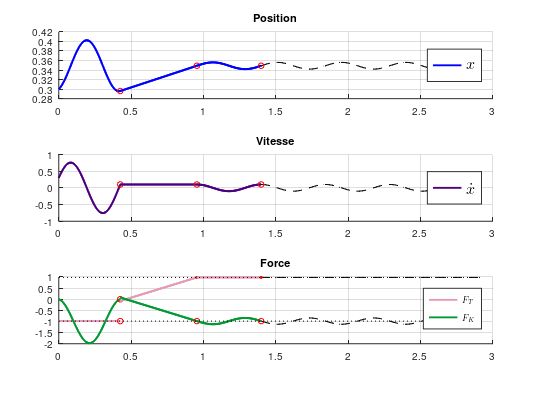
\includegraphics[scale=.6]{CAS2.png}
	\caption{Cas 2}
\end{figure}

\paragraph{Cas 3}
$ $ 
\begin{figure}[h!]
	\centering
	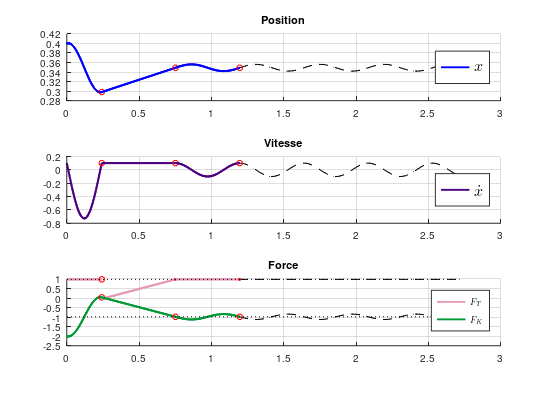
\includegraphics[scale=.75]{CAS3.png}
	\caption{Cas 3}
\end{figure}

\paragraph{Cas 4}
$ $

\begin{figure}[h!]
	\centering
	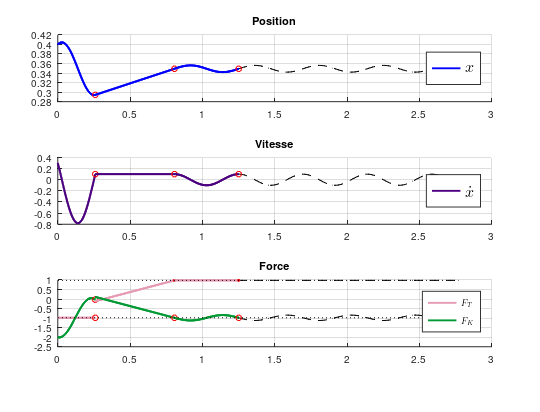
\includegraphics[scale=.75]{CAS4.png}
	\caption{Cas 4}
\end{figure}


\medskip
On remarque qu'ici aussi, après le premier régime d'adhérence, on se retrouve en régime de glissement sans plus jamais en sortir. Le régime d'adhérence vient ici encore "lisser" le problème. 



\end{document}